En el primer sprint se busca identificar cada una de las variables que entran en juego en el sistema, así como su proceso de obtención.. Se debe tener clara la diferencia entre variables de entrada y salida y variables de control.
\subsection{Variables de entrada}
Son las fuentes de suministro de energía al sistema. Habrá un total de tres:
\begin{itemize}
	\item \textbf{Energía fotovoltaica (EF)}\\ Energía procedente de las placas solares. Su valor viene determinado por varios factores, como son el número de módulos fotovoltaicos instalados y la máxima potencia posible en cada momento, \textit{current module power} (CMP). Hace referencia a la potencia de salida, en watios que produce un panel fotovoltaico en condiciones de máxima iluminación solar, con una radiación de aproximadamente 1 kW/m2. Será dependiente de la situación meteorológica del momento, de cuya obtención se hablará mas adelante. Como se puede observar, tendrá un valor máximo de obtención, que representa el tope de energía que podemos obtener de los módulos fotovoltaicos en ese momento.
	\item \textbf{Energía de red (ER)}\\ Energía procedente de la compañía eléctrica como cliente particular. Al contrario que en el caso anterior, no existe un límite superior a la hora de obtener energía de esta fuente.
	\item \textbf{Energía almacenada en batería (EB)}\\ Energía obtenida de la batería de almacenaje, que se ha guardado previamente para su posterior uso cuando el resto de fuentes de entrada tengan un mayor costo. Al igual que la energía fotovoltaica tiene un límite superior y viene determinado por la cantidad de carga de la misma y la profundidad de descarga que se le puede realizar sin resultar perjudicial para su ciclo de vida, que debe ser de un 50\% como máximo.
\end{itemize}

Cómo se ha mencionado, la energía fotovoltaica en una hora t será dependiente de la situación meteorológica de esa hora, algo evidente.\\Para obtener dicha información se utiliza la API oficial de AEMET \cite{Aemet}. Una API (\textit{Application Programming Interface}) es un conjunto de reglas o especificaciones que permite a las aplicaciones proporcionar servicios a otras o comunicarse. Para su uso, se ha debido solicitar un \textbf{API key} ya que es una API cerrada, esto es, su uso está restringido a un conjunto cerrado de clientes. Para realizar una petición a la misma, debe incluirse el \textit{API key} mencionado anteriormente en la url solicitada, así como una serie de parámetros como el código del municipio que se desea consultar. La respuesta a la petición contiene la previsión meteorológica de las próximas 24 horas en ese municipio.\\Para esta funcionalidad se ha creado el módulo \textit{api\_aemet}, que contiene la función \textit{get\_weather}, la cual se muestra en el listado~\ref{lst:aemet}
\begin{lstlisting}[language=Python,float=ht,caption={Función para obtener los valores meteorológicos},label={lst:aemet}]
def get_weather (city):
    weather_buffer = []
    url = const.AEMET_URL.replace('$CITY', city)
    response = requests.get(url)
    data = response.json()

    if data['estado'] == 200:
        url = data['datos']
        response = requests.get(url)
        data = response.json()[0]
        weather_buffer = create_weather_buffer(data)
        return weather_buffer
    return None
\end{lstlisting}
 Nótese que la url para la petición es obtenida como una constante de \textit{const}, alias que hace referencia al módulo de constantes del proyecto: \textit{project\_constants}. Este método realiza una petición a la API mediante la librería \textit{requests}~\cite{Kenn11}, y en caso de obtener un código de éxito (código de estado http 200), procesa la respuesta en la función \textbf{create\_weather\_buffer} y devuelve una lista con los 24 estados meteorológicos, correspondientes a las 24 horas de la simulación, del tipo: ["Despejado", "Poco Nuboso", "Despejado", ..., "Despejado"]\\

Las variables de entrada no son excluyentes, es decir, se puede obtener un tanto por ciento de la energía requerida procedente de cada una de ellas, lo que vendrá determinado por el precio en ese momento de cada una, ya que lo que buscamos es minimizar el gasto producido. A continuación se muestra el modo de determinación de los precios de las variables de entrada en una hora t: \\

	El precio de la energía fotovoltaica se calcula a partir de la inversión realizada en la instalación de los módulos fotovoltaicos y la cantidad de años en los que se desea amortizar dicha inversión. Así, el precio en €/Kw de EF se toma a partir de la fórmula~\ref{eq:costoEF}
	\begin{equation}
          \label{eq:costoEF}
	Costo_{EF} = \frac{coste_{anual}}{promedio^{kw}_{anual}} \textup{\euro}/kw
	\end{equation}
	Siendo el coste anual la cantidad invertida entre el número de años(n) en amortizarla, cómo se puede observar en la fórmula~\ref{eq:inversionEF}
	\begin{equation}
          \label{eq:inversionEF}
	Coste_{anual} = \frac{inversion}{n} \textup{\euro}
	\end{equation}


	El precio de la energía de red es el ya comentado PVPC. Para obtenerlo, se hace uso de la \textbf{API oficial de Red Eléctrica de España (e-sios)} \cite{Ree}. Para su uso se ha debido solicitar un \textit{Token} de acceso que se utiliza en las llamadas a la misma, al tratarse de una API cerrada análogamente al caso de la API de AEMET. Para el procesado de esta API se ha creado el módulo \textit{api\_esios}, que contiene la función \textit{get\_incoming\_prices}, la cuál se muestra en el listado~\ref{lst:esios}

	\begin{lstlisting}[language=Python,float=ht,caption={Función para obtener los valores del precio eléctrico},label={lst:esios}]
	def get_incoming_prices(indicator, start, end):
	   url = const.ESIOS_URL.replace('$INDICATOR', indicator)
	   url = url.replace('$START_DATE', dt.datetime.strftime(start, '%Y/%m/%d'))
	   url = url.replace('$END_DATE', dt.datetime.strftime(end, '%Y/%m/%d'))

	   response = requests.get(url, headers=HEADERS)
	   if response.status_code == 200:
	      data = response.json()
	      price_buffer = create_price_buffer(data, start)
	      return price_buffer
	   return None
	\end{lstlisting}

	Esta función es llamada desde el proyecto con el indicador deseado, que se corresponde con el precio que se desea consultar (en este caso PVPC), cuyo código numérico es obtenido de las constantes del proyecto, al igual que la url necesaria para la petición (ESIOS\_URL), que se forma con los parámetros adecuados y se realiza la petición \textit{get} haciendo uso de la librería \textit{requests}~\cite{Kenn11}. En este caso el \textit{API key} no se concatena en la url, si no que debe incluirse en la cabecera de la petición en un campo específico, ya que se trata de una autenticación por token como tal. Si la petición ha sido exitosa (código de respuesta http 200), la función retornará un \textit{buffer} de tamaño 24, que se corresponde con los valores del PVPC en las 24 horas definidas en la simulación. Para ello llama a \textit{create\_price\_buffer}, que se encargará de generar la lista con los 24 valores del precio solicitado procesando la respuesta recibida de la petición a la API.
	De esta manera se consigue el precio por Kw de la energía de red en cada momento.

	Por último, el precio de la energía de baterías se puede calcular de un modo muy parecido al de la energía fotovoltaica. Hace referencia al coste que supone extraer energía almacenada en la batería y está relacionado con la inversión realizada en la batería~\ref{eq:costoEB}
	\begin{equation}
          \label{eq:costoEB}
	Costo_{EB} = \frac{coste_{anual}}{capacidad_{bat}\cdot182,5} \textup{\euro}/kw
	\end{equation}
	Habiendo obtenido previamente el coste anual de forma similar a la fórmula~\ref{eq:inversionEF}. La constante 182,5 hace referencia al número de días del año (365) multiplicado por 0.5, debido a que no se va a realizar una profundidad de descarga mayor al 50\% de la capacidad total de la batería. El valor obtenido es el precio que supone recoger 1 Kw de la batería.
\subsection{Variables de salida}
Representan las fuentes de consumo de energía del sistema. Habrá un total de cuatro:
\begin{itemize}
	\item \textbf{Consumo del hogar (C)}\\Demanda energética del hogar en cuestión, cuantía que debe ser satisfecha siempre, ya que es el uso de energía que necesita el hogar para su uso cotidiano.
	\item \textbf{Consumo interno del sistema ($ C_{int} $)}\\El sistema propuesto tiene un consumo constante de funcionamiento, cuyo valor se ha estimado en aproximadamente 2 Kw al día, alrededor de unos 0,088 watios por hora. Consta del consumo por funcionamiento de placas fotovoltaicas y realización de carga y descarga de batería.
	\item \textbf{Carga de batería (CB)}\\Cantidad de energía que se almacena en la batería para su posterior uso (almacenaje en batería). Esta variable cobra sentido en el caso de un abaratamiento de alguna fuente de generación de energía, lo que propicia que se obtenga más de la necesitada y se almacene para cuando el precio sea mayor.
	\item \textbf{Vertido al mercado eléctrico (CR)}\\Cantidad de energía que se vende al mercado eléctrico. Como particular, se puede disponer de una instalación fotovoltaica y verter energía a la red eléctrica, aunque es una práctica sujeta a numerosas trabas legales y dificultades en las que no se entrará en el desarrollo de este trabajo fin de grado. Esta energía se vertería al intramercado de red conocido como el mercado SPOT, aquel donde los activos que se compran o venden se entregan al precio de mercado del momento de la compra/venta.
\end{itemize}

Como se puede observar, el vertido al mercado eléctrico es un consumo que tiene un beneficio económico que ha de tenerse en cuenta. Existe una retribución por Kw vertido a la red dependiente del momento del día, ya que como se ha comentado antes, el valor de compra/venta del mercado SPOT varía. Para la obtención de estos valores se vuelve a hacer uso de la ya mencionada API e-sios, proporcionando a la función \textit{get\_incoming\_prices} el indicador del precio SPOT, presente en el fichero de constantes del proyecto. Análogo a la obtención del PVPC, se retorna un buffer con los 24 valores requeridos del precio SPOT correspondientes a las 24 horas a simular.\\

Aunque a priori parezca que el hecho de cargar las baterías no tiene una compensación económica, esto no es del todo correcto. Existe un beneficio económico, aunque no directo, con esta práctica. Puede ser explicado como la cantidad ahorrada por almacenar esa energía y no consumirla, ya que se ha pagado por ella. Este valor puede verse como el mínimo de los precios de las fuentes de generación de energía en el momento de la carga. Veamos un breve ejemplo:\\En la hora t se ha obtenido energía fotovoltaica a un precio de 0,11 € el Kwh. Por otro lado, se ha obtenido energía de la compañía eléctrica contratada a un precio de 0,14 € el Kwh. El beneficio económico indirecto por cargar un Kw de energía en batería en esta hora t será de 0,11 €.

\subsection{Variables de control}
Los valores de las variables definidas anteriormente son los que se intentan optimizar, pero existe otro conjunto de variables conocido como las variables de control. Aunque se denotan como variables, en el caso concreto de una simulación son constantes, ya que sus valores están predefinidos para la simulación del modelo. Este conjunto está formado por los valores de los que dependen las variables de entrada y salida y en función de los que se busca una optimización, y caracterizan tanto la simulación como la situación en una hora determinada.\\
Este conjunto está formado por:
\begin{itemize}
	\item \textbf{Fecha de inicio}\\ Valor que hace referencia al inicio de la simulación. Este valor es representado mediante el módulo datetime de Python. Datetime~\cite{Dtpy} es un módulo de la librería estándar de Python que permite manipular y trabajar con fechas. Este valor será un día y una hora de ese día.
	\item \textbf{Fecha de fin}\\ Corresponde al fin de la simulación. Siempre será 24 horas a partir de la fecha de inicio. Al igual que el anterior, se representa haciendo uso de datetime.
	\item \textbf{Número de módulos fotovoltaicos}\\ El número de módulos fotovoltaicos juega un papel fundamental. A mayor número de módulos, se producirá mas energía, pero mayor deberá ser la inversión para adquirirlos.
	\item \textbf{Precio de un módulo fotovoltaico}\\ En este trabajo el tipo de módulo fotovoltaico sera el se suele usar a nivel particular, de tamaño pequeño, con una potencia nominal en condiciones ideales de 50 watios hora~\ref{fig:pv_module}. Este modulo tiene un precio por unidad de 40 €, por lo tanto este valor tendrá el mismo valor en todas las simulaciones.
          \begin{figure}[!h]
            \centering
            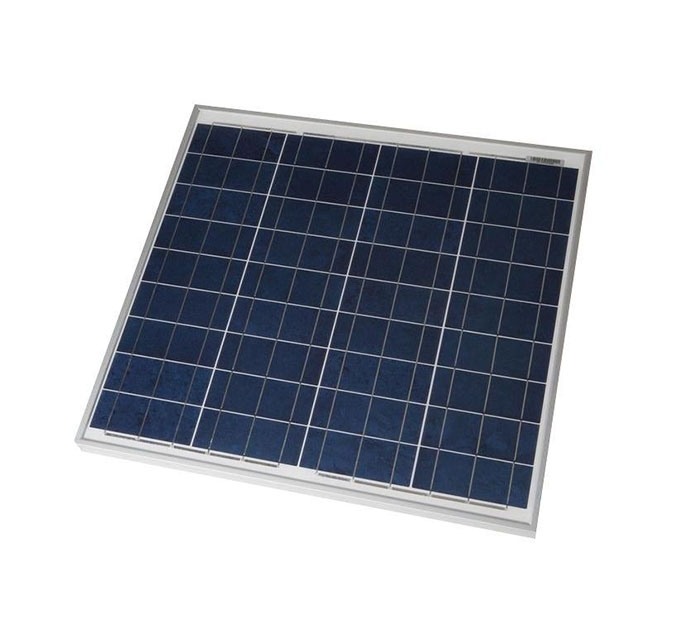
\includegraphics[width=6cm]{figs/panel_solar.jpg}
            \caption{Panel fotovoltaico de 50 W}
            \label{fig:pv_module}
          \end{figure}
	\item \textbf{Años en amortizar la inversión de los módulos fotovoltaicos}\\ El número de años en los que se desea amortizar la inversión realizada en la adquisición de los módulos fotovoltaicos, exclusivamente mediante su uso. Como se ha comentado anteriormente, no es algo trivial ya que determinará en gran medida el precio de extracción de energía fotovoltaica.
	\item \textbf{Precio de la batería}\\ En este trabajo el tipo de batería usado será una batería estacionaria~\ref{fig:bateria} compuesta por plomo abierto y gel. Este tipo de batería esta compuesta por dos vasos de 2V cada uno que disponen de un amplio rango de autonomía y una vida útil bastante larga, alrededor de unos 20 años. Son aconsejadas en instalaciones con un consumo medio (microondas, horno, lavadora, aire acondicionado, etc), es decir, perfectas para un hogar de tamaño normal. Cómo su tensión es de 2V, se debe instalar un total de 6 vasos en serie, al estar la instalación solar a 12V. Su precio es elevado debido a la gran capacidad, siendo un precio de 7900 € el de la obtención de los 6 vasos.
           \begin{figure}[!h]
            \centering
            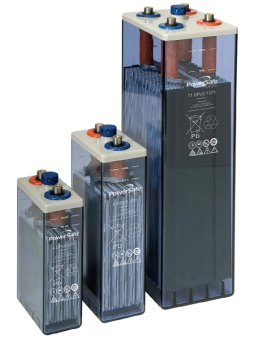
\includegraphics[width=4cm]{figs/bateria.jpg}
            \caption{Batería estacionaria}
            \label{fig:bateria}
          \end{figure}
	\item \textbf{Capacidad de la batería}\\ El tipo de batería usado, es decir, batería estacionaria de 6 vasos, tiene una capacidad total de aproximadamente 21 Kw. La profundidad de descarga de este tipo de batería es aproximadamente del 50\%, esto es, como se comento durante la explicación de las variables de entrada y salida, el tanto por ciento que se puede descargar dicha batería sin resultar perjudicial para su salud y por lo tanto afectar a su ciclo de vida útil.
	\item \textbf{Nivel de carga inicial de la batería}\\ Variable de control que define el estado inicial de la batería a la hora de realizar la simulación del modelo. Esto es la cantidad de energía que tiene almacenada la misma.
	\item \textbf{Años en amortizar la inversión de la batería}\\ Como ocurre en el caso de la inversión fotovoltaica, se debe determinar el número de años en los que se desea realizar la amortización de la inversión por adquirir la batería. Al tratarse de un valor mucho mas elevado debe ser mayor al del caso anterior, ya que si no se dispararía el precio de descargar las baterías y dejaría de ser una entrada a tener en cuenta al no resultar rentable.
\end{itemize}
Con esto quedan identificadas cada una de las variables que entran en juego en el modelo, así como su medio de adquisición.
